Functional analysis defines how \abbr{EWAS} performs its mission from initial observation to warning delivery and long-term system improvement. It describes the main operational flows between the \abbr{GEO} and \abbr{LEO} satellite layers, the ground segment, and the national authority users. The purpose of this section is to clarify the sequence of functions required to detect a potential missile launch, process and validate the event, estimate the threat trajectory and impact area, disseminate an alert, and maintain the system during routine and crisis operations.

\begin{figure}[htbp]
    \centering
    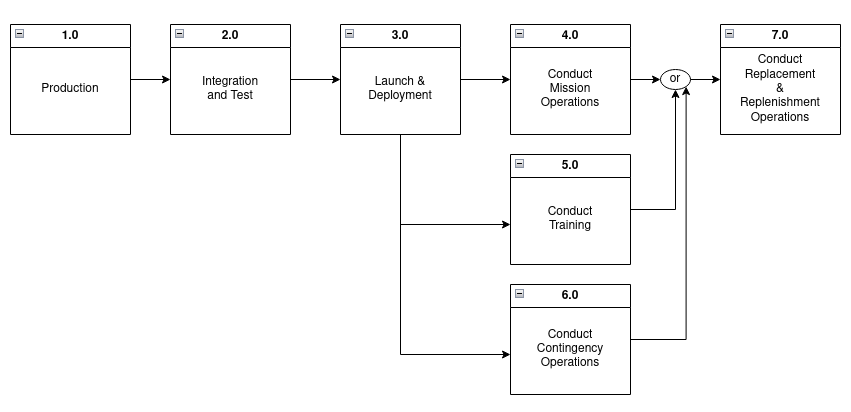
\includegraphics[width=0.9\textwidth]{Figures/general_flow_2.png}
    \caption{Top Level Flow}
    \label{fig:general-flow}
\end{figure}




\subsection{Primary Threat Detection and Warning Flow}
The primary objective is to identify launch events that may threaten the Baltic region, including launches outside that region, assess the potential threat and communicate actionable preliminary warnings to authorized authorities. This mission is conducted in accordance with the functional flow shown in Figure~\ref{fig:mission-operation-flow}.

The baseline constellation includes six \abbr{GEO} satellites operating at 35,786~km and 72 high-inclination \abbr{LEO} satellites operating at 1,000~km across 8 orbital planes, interconnected by a mandatory Space Segment Inter-Satellite Link (\abbr{ISL}) network (optical/\abbr{RF} \abbr{ISL} mesh in \abbr{LEO} and cross-layer \abbr{GEO}--\abbr{LEO} relay links). The \abbr{GEO} layer provides initial wide-area thermal-event detection and onboard preliminary filtering, while the \abbr{LEO} layer provides agile follow-on stereoscopic tracking.

After the initial thermal event is identified, the detecting \abbr{GEO} satellite reports the event to the Ground Segment (R-042). The Ground Segment selects two suitable \abbr{LEO} satellites according to event location, observation geometry, and link routing (R-043), and transmits tracking commands via direct ground-station links or mandatory Space Segment \abbr{ISL} relay paths (R-044). The two cued \abbr{LEO} satellites rapidly orient their sensors using agile optical Line-of-Sight (LOS) steering, acquire complementary stereoscopic observations, exchange timestamped LOS observation vectors via mandatory \abbr{ISL} to compute an onboard preliminary 3D trajectory estimate (R-023), and downlink both the encrypted timestamped LOS observation packages (with covariance/uncertainty metadata) and the preliminary trajectory estimate to the Ground Segment.

The Ground Station Network securely receives and forwards the downlinked data, and the central Ground Segment Data Processing System performs authoritative multi-sensor fusion (R-026, R-027) to calculate a refined trajectory and probabilistic impact-area (Instantaneous Impact Point --- IIP) estimate (R-012). Once this authoritative two-\abbr{LEO} assessment is completed, the Early Warning System automatically dispatches the first preliminary warning to appropriate authorized national authorities (R-045). The Mission Control Center presents the event for subsequent operator confirmation, updating, or cancellation (R-046), and the Data Archiving System stores all relevant event and warning records in accordance with R-004 and R-047. Mandatory \abbr{ISL} routing and fast payload LOS steering enable the architecture to satisfy the $\le 60\text{-second}$ end-to-end warning latency budget from initial \abbr{GEO} detection to external authority interface delivery (R-011).


\begin{figure}[htbp]
    \centering
    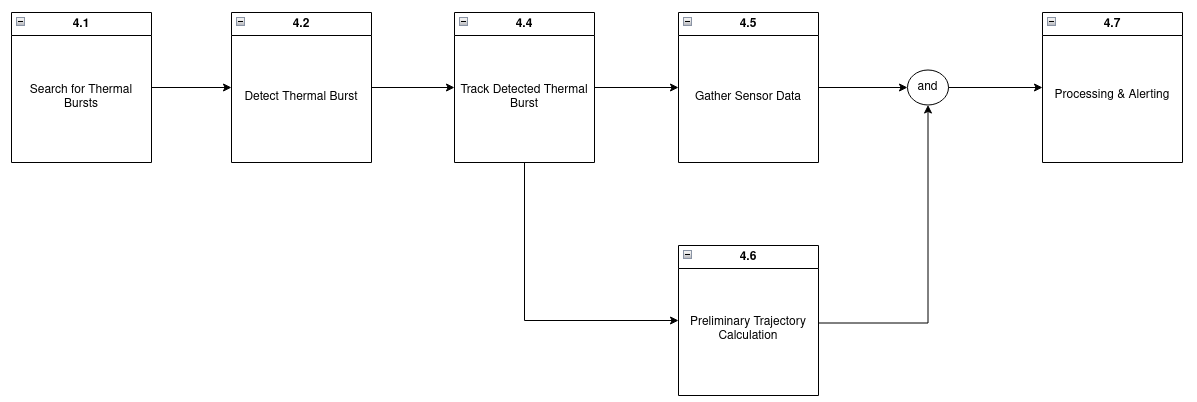
\includegraphics[width=0.9\textwidth]{Figures/warning_flow_2.png}
    \caption{Second Level Flow}
    \label{fig:mission-operation-flow}
\end{figure}


\subsection{Data Management and Continuous Improvement Flow}

This flow operates asynchronously to the warning path and uses historical data solely for the technical purposes authorized by R-004.

\begin{itemize}
    \item Archive the applicable raw sensor readings, onboard processing logs, received telemetry, processing outputs, preliminary and updated warning products, delivery acknowledgements and review records in encrypted Ground Segment storage.
    \item Retrieve historical event data for authorized post-event technical analysis, lessons-learned review, and missile characterization.
    \item Use archived data to refine detection, classification, denoising, tracking, and impact-area estimation algorithms.
    \item Reduce false alarm rates by comparing confirmed missile events with non-threat thermal signatures such as solar bursts and Earth background noise.
    \item Prepare validated software and algorithm updates for the space segment and ground processing center.
    \item Securely uplink approved updates to satellites and deploy them to the ground segment during planned operation and maintenance windows.
    \item Share authorized operational warning products with national authority recipients; do not assume general external dissemination of historical archive contents beyond the purposes permitted by R-004.
\end{itemize}

\subsection{System Maintenance and Support Flow}

This background operational loop ensures that \abbr{EWAS} maintains high availability, reliable coverage, and stable performance during both routine operation and crisis conditions.

\begin{itemize}
    \item Continuously monitor satellite health and status telemetry from the space segment.
    \item Verify communication links between \abbr{GEO} satellites, \abbr{LEO} satellites, ground stations, and national authority interfaces.
    \item Perform attitude and orbit control to maintain required satellite pointing, orbital positioning, and coverage of the monitored region.
    \item Regulate spacecraft power and thermal conditions using the Electrical Power System (\abbr{EPS}) and Thermal Control System (\abbr{TCS}).
    \item Detect subsystem anomalies and initiate fault-management procedures when degraded performance is observed.
    \item Maintain ground segment hardware, processing infrastructure, databases, and operator consoles.
    \item Apply tested software patches and configuration updates to preserve redundant and uninterrupted operations.
\end{itemize}